
% !TeX root = Asparsi.tex
% !BIB TS-program = biber
% !TeX encoding = UTF-8
% !TeX spellcheck = it_IT
\chapter{Triangolo}\label{ch:triangolo}
\begin{thm}[Posizione punto circonferenza]\label{thm:Posizione-punto-circonferenza}
Data una circonferenza $C$ di diametro$AB$, valgono le seguenti affermazioni
\begin{itemize}
	\item Un punto $P$ appartiene a $C$ se e solo se $A\hat{P}B$ è retto.
	\item Un punto $P$ è interno a $C$ se e solo se $A\hat{P}B$ è ottuso.
	\item Un punto $P$ è esterno a $C$ se e solo se $A\hat{P}B$ è acuto
\end{itemize}
\end{thm}\index{Circonferenza}
\begin{proof} Consideriamo i vari casi\newline
	\begin{itemize}
		\item Un punto $P$ appartiene a $C$ se e solo se $A\hat{P}B$ è retto.\newline
		Se il punto è sulla circonferenza come nella~\cref{fig:circonferenza1} l'angolo in $\hat{P}$ è la metà di un angolo piatto quindi è retto. 
		\item Un punto $P$ è interno a $C$ se e solo se $A\hat{P}B$ è ottuso.\newline Consideriamo la~\cref{fig:circonferenza2}. Se il punto $P$ è interno prolunghiamo $AP$ in modo che incontri in $Q$ la circonferenza. Il Triangolo $AQB$ è retto in$Q$. L'angolo $A\hat{P}B$ è somma di $P\hat{Q}B$ e $P\hat{B}Q$, quindi è ottuso.
		\item Un punto $P$ è esterno a $C$  se e solo se $A\hat{P}B$ è acuto.\newline
		Prendiamo un punto $P$ punto esterno alla circonferenza $C$ come nella~\cref{fig:circonferenza3}. Se $AP$ è secante a $C$ in  $Q$ l'angolo $A\hat{Q}B$ è retto ed è la somma di $Q\hat{P}B$ e $Q\hat{B}P$. Quindi $A\hat{P}B$ è acuto.
	\end{itemize}
\end{proof}
\begin{figure}
	\centering
	\documentclass[10pt]{standalone}
\usepackage[utf8]{inputenc}
\usepackage{pgf,tikz,pgfplots}
\pgfplotsset{compat=1.15}
\usepackage{mathrsfs}
\usetikzlibrary{arrows}
\pagestyle{empty}
\begin{document}

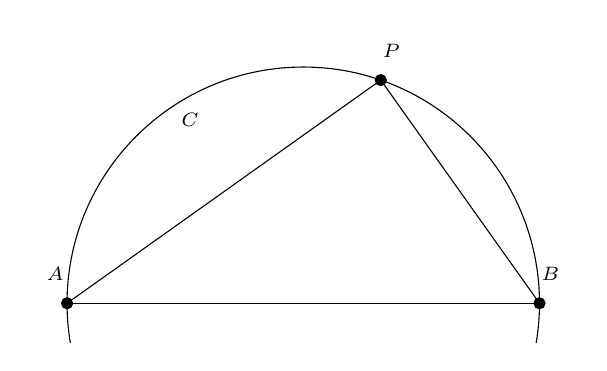
\begin{tikzpicture}[line cap=round,line join=round,>=triangle 45,x=1.0cm,y=1.0cm]

\clip(-0.5,-0.5) rectangle (6.5,3.5);
\draw  (3.,0.) circle (3.cm);
\draw  (0.,0.)-- (6.,0.);
\draw  (0.,0.)-- (3.9844047938229687,2.833892588278243);
\draw  (3.9844047938229687,2.833892588278243)-- (6.,0.);
\begin{scriptsize}
\draw [fill=black] (0.,0.) circle (2.0pt);
\draw (-0.15,0.37) node {$A$};
\draw [fill=black] (6.,0.) circle (2.0pt);
\draw (6.14,0.37) node {$B$};
\draw (1.56,2.33) node {$C$};
\draw [fill=black] (3.9844047938229687,2.833892588278243) circle (2.0pt);
\draw (4.12,3.21) node {$P$};
\end{scriptsize}
\end{tikzpicture}
\end{document}
	\caption{Posizione punto circonferenza, angolo retto}
	\label{fig:circonferenza1}
\end{figure}
\begin{figure}
	\centering
	\documentclass[10pt]{standalone}
\usepackage[utf8]{inputenc}
\usepackage{pgf,tikz,pgfplots}
\pgfplotsset{compat=1.15}
\usepackage{mathrsfs}
\usetikzlibrary{arrows}
\pagestyle{empty}
\begin{document}

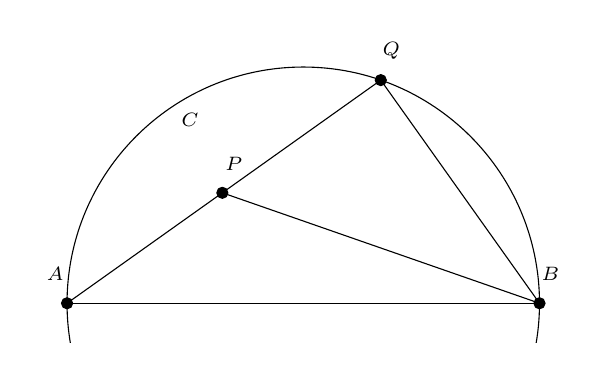
\begin{tikzpicture}[line cap=round,line join=round,>=triangle 45,x=1.0cm,y=1.0cm]

\clip(-0.5,-0.5) rectangle (6.5,3.5);
\draw  (3.,0.) circle (3.cm);
\draw  (0.,0.)-- (6.,0.);
\draw  (0.,0.)-- (3.9844047938229687,2.833892588278243);
\draw  (3.9844047938229687,2.833892588278243)-- (6.,0.);
\draw  (1.9722601452080204,1.4027624442994568)-- (6.,0.);
\begin{scriptsize}
\draw [fill=black] (0.,0.) circle (2.0pt);
\draw (-0.15,0.37) node {$A$};
\draw [fill=black] (6.,0.) circle (2.0pt);
\draw (6.14,0.37) node {$B$};
\draw (1.56,2.33) node {$C$};
\draw [fill=black] (3.9844047938229687,2.833892588278243) circle (2.0pt);
\draw (4.12,3.21) node {$Q$};
\draw [fill=black] (1.9722601452080204,1.4027624442994568) circle (2.0pt);
\draw (2.12,1.77) node {$P$};
\end{scriptsize}

\end{tikzpicture}
\end{document}
	\caption{Posizione punto circonferenza, angolo ottuso}
	\label{fig:circonferenza2}
\end{figure}
\begin{figure}
	\centering
	\documentclass[10pt]{standalone}
\usepackage[utf8]{inputenc}
\usepackage{pgf,tikz,pgfplots}
\pgfplotsset{compat=1.15}
\usepackage{mathrsfs}
\usetikzlibrary{arrows}
\pagestyle{empty}
\begin{document}

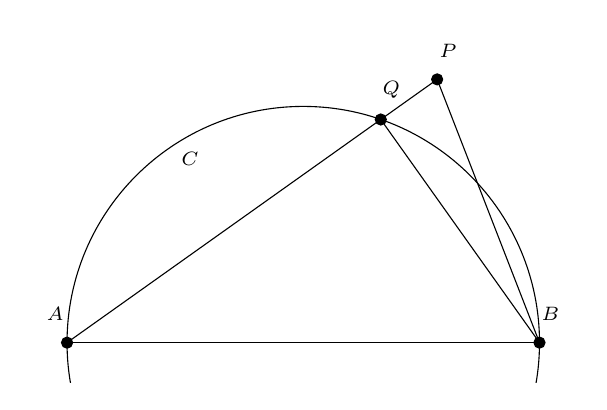
\begin{tikzpicture}[line cap=round,line join=round,>=triangle 45,x=1.0cm,y=1.0cm]

\clip(-0.5,-0.5) rectangle (6.5,4.);
\draw  (3.,0.) circle (3.cm);
\draw  (0.,0.)-- (6.,0.);
\draw  (0.,0.)-- (3.9844047938229687,2.833892588278243);
\draw  (3.9844047938229687,2.833892588278243)-- (6.,0.);
\draw  (4.700426856560177,3.3431605270630866)-- (6.,0.);
\draw  (4.700426856560177,3.3431605270630866)-- (3.9844047938229687,2.833892588278243);
\begin{scriptsize}
\draw [fill=black] (0.,0.) circle (2.0pt);
\draw[color=black] (-0.15,0.37) node {$A$};
\draw [fill=black] (6.,0.) circle (2.0pt);
\draw[color=black] (6.14,0.37) node {$B$};
\draw[color=black] (1.56,2.33) node {$C$};
\draw [fill=black] (3.9844047938229687,2.833892588278243) circle (2.0pt);
\draw[color=black] (4.12,3.21) node {$Q$};
\draw [fill=black] (4.700426856560177,3.3431605270630866) circle (2.0pt);
\draw[color=black] (4.84,3.71) node {$P$};
\end{scriptsize}

\end{tikzpicture}
\end{document}
	\caption{Posizione punto circonferenza, angolo acuto}
	\label{fig:circonferenza3}
\end{figure}
\begin{defn}[Ceviana]\label{defn:ceviana1}
Una Ceviana è un segmento che congiunge un vertice di un triangolo con il suo lato opposto.
\end{defn}\index{Triangolo!ceviana}\index{Ceviana}
\section{Teorema di Stewart}\label{sec:teorema-di-stewart}
\begin{thm}[Teorema di Stewart]\label{thm:Stewart}
Dato un triangolo $ABC$ colleghiamo un vertice con il lato opposto come nella figura~\cref{fig:stewart1} allora vale la relazione 
\begin{align*}
c^2y+b^2x=&a(t^2+xy)\\     
a^2y+c^2x=&b(l^2+xy)\\        
b^2y+a^2x=&c(m^2+xy)
\end{align*}
\end{thm}\index{Triangolo!teorema di Stewart}
\begin{figure}
	\centering
	\documentclass[10pt]{standalone}
\usepackage[utf8]{inputenc}
\usepackage{pgf,tikz,pgfplots}
\pgfplotsset{compat=1.15}
\usepackage{mathrsfs}
\usetikzlibrary{arrows}
\pagestyle{empty}
\begin{document}

\begin{tikzpicture}[line cap=round,line join=round,>=triangle 45,x=1.0cm,y=1.0cm]
\clip(0.,-0.8) rectangle (10.5,5.5);

\draw  (4.,5.)-- (10.,0.) node [midway,above] {$c$};
\draw  (10.,0.)-- (6.,0.)node [midway,below] {$y$};
\draw  (1.,0.)-- (6.,0.)node [midway,below] {$x$};
\draw  (1.,0.)-- (4.,5.)node [midway,above] {$b$};
\draw  (4.,5.)-- (6.,0.)node [midway,above] {$t$};

\draw [fill=black] (4.,5.) circle (2.0pt);
\draw[color=black] (4.14,5.33) node {$A$};
\draw [fill=black] (1.,0.) circle (2.0pt);
\draw[color=black] (0.82,-0.33) node {$B$};
\draw [fill=black] (10.,0.) circle (2.0pt);
\draw[color=black] (9.92,-0.33) node {$C$};
\draw [fill=black] (6.,0.) circle (2.0pt);
\draw[color=black] (6.02,-0.33) node {$P$};
\draw[color=black] (6.02,-0.5) node {$a$};
\end{tikzpicture}
\end{document}
	\caption{Teorema di Stewart}
	\label{fig:stewart1}
\end{figure}
\begin{proof}
Poniamo
\begin{align*}
AB=&c&&AC=b&&BC=a\\
AP=&t&&BP=x&&PC=y
\end{align*}
Indichiamo con $\alpha$ l'angolo $A\hat{P}B$ Applichiamo il teorema di Carnot\index{Triangolo!Carnot} ai triangoli $APB$ e $PCA$ avremo 
\begin{align*}
c^2=&t^2+x^2-2xt\cos\alpha\\
b^2=&t^2+y^2-2ty\cos(\pi-\alpha)\\
c^2=&t^2+x^2-2xt\cos\alpha\\
b^2=&t^2+y^2+2ty\cos\alpha\\
\intertext{Moltiplichiamo la prima per $y$ e la seconda per $x$ ottengo}
c^2y=&t^2y+x^2y-2xyt\cos\alpha\\
b^2x=&t^2x+y^2x+2xyt\cos\alpha\\
\intertext{sommando otteniamo}
c^2y+b^2x=&t^2y+x^2y+t^2x+y^2x\\
c^2y+b^2x=&t^2(x+y)+xy(x+y)\\
c^2y+b^2x=&(x+y)(t^2+xy)\\
c^2y+b^2x=&a(t^2+xy)\\
\end{align*}
come si volevasi dimostrare
\end{proof}\index{Triangolo!Carnot}\index{Triangolo!ceviana}
\begin{cor}[Lunghezza ceviana]\label{cor:ceviana1}
In un trangolo le ceviane hanno lunhezza:
\begin{align*}
l=&\sqrt{\dfrac{a^2y-x(by-c^2)}{b}}\\
m=&\sqrt{\dfrac{b^2y-x(cy-a^2)}{c}}\\
t=&\sqrt{\dfrac{c^2y-x(ay-b^2)}{a}}\\
\end{align*}
\end{cor}
\section{Circocentro}\label{sec:circocentro}
\begin{defn}[Circonferenza circoscritta]\label{defn:CircCirc1}
Dato un triangolo, una circonferenza circoscritta è una circonferenza che passa per i vertici del triangolo\index{Triangolo!circonferenza!circoscritta}\index{Circonferenza!circoscritta}
\end{defn}
\begin{figure}
	\centering
\includestandalone{geometria/circumcerchio}
	\caption{Circonferenza circonscritta}
	\label{fig:circumcerchio}
\end{figure}
\begin{defn}[Circocentro]\label{defn:Circocentro1}
Il circocentro è il centro della circonferenza circonscritta. \index{Triangolo!circocentro}
\end{defn}
\begin{thm}[Assi dei lati e circocentro]\label{thm:CircoAsse1}
Il circocentro è il punto di incontro degli assi del segmento.\index{Triangolo!circocentro}\index{Triangolo!asse!lato}\index{Circocentro!triangolo}
\end{thm}
\begin{proof}
	Consideriamo il triangolo $ABC$ della figura~\cref{fig:circumcerchio2}, per comodità poniamo il vertice $A$ nell'origine degli assi e il vertice $B$ sull'asse delle $x$. Determiniamo la circonferenza che passa per i tre vertici.
	\begin{align*}
	\intertext{Considero la circonferenza generica}
	x^2+y^2+ax+by+c=&0\\
	\intertext{Passaggio per $A(0,0)$ }
	c=&0\\
	\intertext{Passaggio per $B(s,0)$}
	s^2+as+c=0\\
	\intertext{Passaggio per $C(t,r)$}
	t^2+r^2+at+br+c=&0\\
	\intertext{Risolvendo il sistema otteniamo}
	\begin{cases}	
		a=-s\\
		b=-\dfrac{t^2+r^2-ts}{r}\\
		c=0
	\end{cases}&\\
	\intertext{L'equazione cercata è}
	x^2+y^2-sx-\dfrac{t^2+r^2-ts}{r}y=&0
	\intertext{Il centro $D$ ha coordinate:}
	\begin{cases}
	x=\dfrac{s}{2}\\ \\
	y=\dfrac{t^2+r^2-ts}{2r}\\
	\end{cases}&\\
		\end{align*}
	Troviamo l'intersezione degli assi dei lati
	\begin{align*}
	\intertext{L'asse del lato $AB$ ha equazione}
	x=&\dfrac{s}{2}\\
	\intertext{Per l'asse del lato $BC$ procediamo come segue:}
	(x-s)^2+y^2=&(x-t)^2+(x-r)^2\\
	x(2t-2s)+2ry-t^2-r^2+s^2=&0\\
	y=&\dfrac{x(s-t)}{r}+\dfrac{t^{2}+r^{2}-s^{2}}{2r}
	\intertext{Risolvendo il sistema otteniamo}
	&\begin{cases}
	x=\dfrac{s}{2}\\ \\
	y=\dfrac{t^2+r^2-ts}{2r}\\
	\end{cases}
	\end{align*}
	Da cui la tesi.
\end{proof}
\begin{proof}
	Consideriamo il triangolo $ABC$ della figura~\cref{fig:circumcerchio2}, per comodità poniamo il vertice $A$ nell'origine degli assi e il vertice $B$ sull'asse delle $x$. Determiniamo la circonferenza che passa per i tre vertici.
	\begin{align*}
	\intertext{Considero la circonferenza generica}
	x^2+y^2+ax+by+c=&0\\
	\intertext{Passaggio per $A(0,0)$ }
	c=&0\\
	\intertext{Passaggio per $B(s,0)$}
	s^2+as+c=0\\
	\intertext{Passaggio per $C(t,r)$}
	t^2+r^2+at+br+c=&0\\
	\intertext{Risolvendo il sistema con il metodo di Cramer}
\Delta=&\begin{vmatrix}
0&0&1\\
s&0&1\\
t&r&1\\
\end{vmatrix}=rs\\
\Delta_a=&\begin{vmatrix}
0&0&1\\
-s^2&0&1\\
-t^2-r^2&r&1\\
\end{vmatrix}=-rs^2\\
\Delta_b=&\begin{vmatrix}
0&0&1\\
s&-s^2&1\\
t&-t^2-r^2&1\\
\end{vmatrix}=-s(t^2-st+r^2)\\
\Delta_c=&\begin{vmatrix}
0&0&0\\
s&0&-s^2\\
t&r&-t^2-r^2\\
\end{vmatrix}=0\\
a=&\dfrac{\Delta_a}{\Delta}=-\dfrac{rs^2}{rs}=-s\\
b=&\dfrac{\Delta_b}{\Delta}=-\dfrac{s(t^2-st+r^2)}{rs}=-\dfrac{t^2-st+r^2}{r}\\
c=&\dfrac{\Delta_c}{\Delta}=-\dfrac{0}{rs}=0
	\intertext{L'equazione cercata è}
&x^2+y^2-sx-\dfrac{t^2+r^2-ts}{r}y=0\\
\intertext{Il centro $D$ ha coordinate:}
&	\begin{cases}
x=\dfrac{s}{2}\\ \\
y=\dfrac{t^2+r^2-ts}{2r}\\
\end{cases}\\
	\end{align*}
	Troviamo l'intersezione degli assi dei lati
	\begin{align*}
	\intertext{L'asse del lato $AB$ ha equazione}
	x=&\dfrac{s}{2}\\
	\intertext{Per l'asse del lato $BC$ procediamo come segue:}
	(x-s)^2+y^2=&(x-t)^2+(x-r)^2\\
	2x(s-t)-2ry=&s^2-r^2-t^2
	\intertext{Risolvendo il sistema otteniamo}
	\Delta=&\begin{vmatrix}
	2(s-t)&-2r\\
	1&0\\
	\end{vmatrix}=2r\\
	\Delta_x=&\begin{vmatrix}
	s^2-r^2-t^2&-2r\\
	\dfrac{s}{2}&0\\
	\end{vmatrix}=rs\\
	\Delta_y=&\begin{vmatrix}
	2(s-t)&s^2-r^2-t^2\\
	1&0\\
	\end{vmatrix}=t^2+r^2-st\\
	x=&\dfrac{\Delta_x}{\Delta}=\dfrac{rs}{2r}=\dfrac{s}{2}\\
	y=&\dfrac{\Delta_y}{\Delta}=\dfrac{t^2+r^2-st}{2r}\\
	\end{align*}
	Da cui la tesi.
\end{proof}
\begin{figure}
	\centering
	\includestandalone{geometria/circumcerchio2}
	\caption{Circocentro ed assi segmento}
	\label{fig:circumcerchio2}
\end{figure}
\begin{cor}[Triangolo rettangolo]\label{cor:CircoAsse1}
	In un triangolo rettangolo il circocentro è il punto medio dell'ipotenusa.\index{Triangolo!rettangolo!circocentro}\index{Circocentro!triangolo!rettangolo}
\end{cor}
\begin{proof}
	Dal \cref{thm:CircoAsse1} sappiamo che il circocentro ha coordinate
	\[	\begin{cases}
	x=\dfrac{s}{2}\\ \\
	y=\dfrac{t^2+r^2-ts}{2r}\\
	\end{cases}\]
	Se come nella figura~\cref{fig:circumcerchio3} il triangolo è retto in $B$ quindi le coordinate del punto $C$ diventano $C(s,r)$ e di conseguenza quelle del punto $D$ si trasformano in 	\[\begin{cases}
	x=\dfrac{s}{2}\\ \\
	y=\dfrac{s^2+r^2-s^2}{2r}=\dfrac{r}{2}\\
	\end{cases}\]Per verificare che il punto $D$ è sull'ipotenusa\index{Triangolo!rettangolo!ipotenusa} basta trovare l'equazione di questa. Banalmente l'ipotenusa ha equazione:
	\begin{align*}
	y=&\dfrac{r}{s}x\\
	\intertext{sostiuendo le coordinate del centro $D$}
	\dfrac{r}{2}=&\dfrac{r}{2}
	\end{align*}
	Da cui la tesi.
\end{proof}
\begin{figure}
	\centering
	\includestandalone{geometria/circumcerchio3}
	\caption{Circocentro e triangolo rettangolo}
	\label{fig:circumcerchio3}
\end{figure}
\begin{cor}[Triangolo ottusangolo]\label{cor:CircoAsse2}
	In un triangolo ottusangolo il circocentro è esterno al triangolo.\index{Triangolo!ottusangolo!circocentro}\index{Circocentro!triangolo!ottusangolo}
\end{cor}
\begin{figure}
	\centering
	\documentclass[10pt]{standalone}
\usepackage[utf8]{inputenc}
\usepackage{pgf,tikz,pgfplots}
\pgfplotsset{compat=1.15}
\usepackage{mathrsfs}
\usetikzlibrary{arrows}
\pagestyle{empty}
\begin{document}

\begin{tikzpicture}[line cap=round,line join=round,>=triangle 45,x=1.0cm,y=1.0cm]
\begin{axis}[
x=1.0cm,y=1.0cm,
axis lines=middle,
xmin=-5.0,
xmax=13.5,
ymin=-6.0,
ymax=9.0,
ticks=none,]
\clip(-5.,-6.) rectangle (13.5,9.);
%\fill[fill=black,fill opacity=0.1] (0.,0.) -- (7.,0.) -- (4.226204810235532,7.183752003695065) -- cycle;
\draw  (0.,0.)-- (7.,0.);
\draw  (7.,0.)-- (4.226204810235532,7.183752003695065);
\draw  (4.226204810235532,7.183752003695065)-- (0.,0.);
\draw [domain=-5.:13.5] plot(\x,{(-0.-0.8680615969584151*\x)/0.49645650754724296});
\draw [domain=-5.:13.5] plot(\x,{(-0.--0.49645650754724296*\x)/0.8680615969584151});
\draw [domain=-5.:13.5] plot(\x,{(-5.772776669005928--0.8246823812865612*\x)/0.5655961191482194});
\draw [domain=-5.:13.5] plot(\x,{(-3.9591728340375356--0.5655961191482194*\x)/-0.8246823812865612});
\draw [domain=-5.:13.5] plot(\x,{(-7.504483873118455--0.08155333557201537*\x)/-0.9966689788776805});
\draw [domain=-5.:13.5] plot(\x,{(--3.6262682949219074-0.9966689788776805*\x)/-0.08155333557201537});
\begin{scriptsize}
\draw [fill=black] (0.,0.) circle (2.0pt);
\draw (0.2,0.7) node {$A$};
\draw [fill=black] (7.,0.) circle (2.0pt);
\draw (7.2,0.7) node {$B$};
\draw [fill=black] (4.226204810235532,7.183752003695065) circle (2.0pt);
\draw (4.5,7.8) node {$C$};
\draw [fill=black] (-4.517678489481885,7.899228118691028) circle (2.0pt);
\draw (-4.2,8.4) node {$D$};
\draw [fill=black] (3.1829859367448132,-5.565498313231292) circle (2.0pt);
\draw (3.4,-5.0) node {$E$};
\draw [fill=black] (11.517678489481884,6.587120612149493) circle (2.0pt);
\draw (11.8,7.2) node {$F$};
\draw [fill=black] (3.817014063255187,2.1830034616692773) circle (2.0pt);
\draw (4.1,2.8) node {$G$};
\end{scriptsize}
\end{axis}
\end{tikzpicture}
\end{document}
	\caption{Incentro di un triangolo}
	\label{fig:incentro1}
\end{figure}
\section{Incentro}\label{sec:incentro}
\begin{defn}[Incentro]\label{defn:incentro1}
L'incentro è il punto di intersezione delle bisettrici di un triangolo
\end{defn}\index{Triangolo!incentro}\index{Incentro!triangolo}\index{Triangolo!bisettrice}
\begin{thm}[Incentro]\label{thm:incentro1}
	Le tre bisettrici si incontrano in un punto detto incentro.
\end{thm}
%\begin{proof}
%	Consideriamo la~\cref{fig:incentro1}. Poniamo $A(0,0)$, $B(s,0)$ e $C(t,r)$
%	\begin{align*}
%	\intertext{La retta $AC$ ha equazione:}
%	xr+y(r-t)=&0
%	\intertext{La retta $AB$ ha equazione:}	
%	y=&0
%	\intertext{La retta $BC$ ha equazione:}
%	xr+y(s-t)-sr=&0
%	\intertext{La bisettrice tra $AC$ e $AB$ è:}
%	\dfrac{xr+y(r-t)}{\sqrt{r^2+(r-t)^2}}=&\pm y
%	\intertext{La bisettrice tra $AB$ e $BC$ è:}
%	\dfrac{xr+y(s-t)-sr}{\sqrt{r^2+(s-t)^2}}=&\pm y
%	\intertext{Poniamo}
%	a=&\sqrt{r^2+(r-t)^2}\\
%	b=&\sqrt{r^2+(s-t)^2}
%	\intertext{otteniamo quattro sistemi}
%	&\begin{cases}
%\dfrac{xr+y(r-t)}{a}=\pm y\\
%\dfrac{xr+y(s-t)-sr}{b}=\pm y
%	\end{cases}\\
%	\intertext{il primo}
%	&\begin{cases}
%	\dfrac{xr+y(r-t)}{a}=y\\
%	\dfrac{xr+y(s-t)-sr}{b}=y
%	\end{cases}\\
%	\intertext{che ha per soluzione}
%	&\begin{cases}
%	x=\dfrac{s(a-r+t)}{a-b-r+s}\\
%	y=\dfrac{rs}{a-b-r+s}
%	\end{cases}\\
%		\intertext{il secondo}
%	&\begin{cases}
%	\dfrac{xr+y(r-t)}{a}=y\\
%	\dfrac{xr+y(s-t)-sr}{b}=-y
%	\end{cases}\\
%	\intertext{che ha per soluzione}
%	&\begin{cases}
%	x=\dfrac{s(a-r+t)}{a+b-r+s}\\
%	y=\dfrac{rs}{a+b-r+s}
%	\end{cases}\\
%			\intertext{il terzo}
%	&\begin{cases}
%	\dfrac{xr+y(r-t)}{a}=-y\\
%	\dfrac{xr+y(s-t)-sr}{b}=y
%	\end{cases}\\
%	\intertext{che ha per soluzione}
%	&\begin{cases}
%	x=\dfrac{s(a+r-t)}{a+b+r-s}\\
%	y=-\dfrac{rs}{a+b+r-s}
%	\end{cases}\\
%		\intertext{il quarto}
%	&\begin{cases}
%	\dfrac{xr+y(r-t)}{a}=-y\\
%	\dfrac{xr+y(s-t)-sr}{b}=-y
%	\end{cases}\\
%	\intertext{che ha per soluzione}
%	&\begin{cases}
%	x=\dfrac{s(a+r-t)}{a-b+r-s}\\
%	y=-\dfrac{rs}{a-b+r-s}
%	\end{cases}\\
%	\intertext{La bisettrice tra $AC$ e $AB$ è:}
%	\dfrac{xr+y(r-t)}{\sqrt{r^2+(r-t)^2}}=&\pm y
%	\intertext{La bisettrice tra $AC$ e $CB$ è:}
%	\dfrac{xr+y(r-t)}{\sqrt{r^2+(r-t)^2}}=&\pm\dfrac{xr+y(s-t)-sr}{\sqrt{r^2+(s-t)^2}}
%	\intertext{Poniamo}
%	a=&\sqrt{r^2+(r-t)^2}\\
%	b=&\sqrt{r^2+(s-t)^2}
%	\intertext{otteniamo quattro sistemi}
%	&\begin{cases}
%	\dfrac{xr+y(r-t)}{a}=\pm y\\
%	\dfrac{xr+y(r-t)}{a}=\pm\dfrac{xr+y(s-t)-sr}{b}
%	\end{cases}\\
%	\intertext{il primo}
%	&\begin{cases}
%	\dfrac{xr+y(r-t)}{a}=y\\
%	\dfrac{xr+y(r-t)}{a}=\dfrac{xr+y(s-t)-sr}{b}
%	\end{cases}\\
%	\intertext{che ha per soluzione}
%	&\begin{cases}
%	x=\dfrac{s(a-r+t)}{a-b-r+s}\\
%	y=\dfrac{rs}{a-b-r+s}
%	\end{cases}\\
%		\intertext{il secondo}
%	&\begin{cases}
%	\dfrac{xr+y(r-t)}{a}=y\\
%	\dfrac{xr+y(r-t)}{a}=-\dfrac{xr+y(s-t)-sr}{b}
%	\end{cases}\\
%	\intertext{che ha per soluzione}
%	&\begin{cases}
%	x=\dfrac{s(a-r+t)}{a+b-r+s}\\
%	y=\dfrac{rs}{a+b-r+s}
%	\end{cases}\\
%	\end{align*}
%\end{proof}
\section{Ortocentro}\label{sec:ortocentro}
\begin{defn}[Ortocentro]\label{defn:ortocentro1}
	L'ortocentro è il punto di intersezione delle altezze di un triangolo \index{Triangolo!ortocentro}\index{Ortocentro!triangolo}
\end{defn}
\begin{thm}[Ortocentro]\label{thm:ortocentro1}
	Le altezze di un triangolo passano tutte per lo stesso punto
\end{thm}
\begin{figure}
	\centering
	\documentclass[10pt]{standalone}
\usepackage[utf8]{inputenc}
\usepackage{pgf,tikz,pgfplots}
\pgfplotsset{compat=1.15}
\usepackage{mathrsfs}
\usetikzlibrary{arrows}
\pagestyle{empty}
\begin{document}

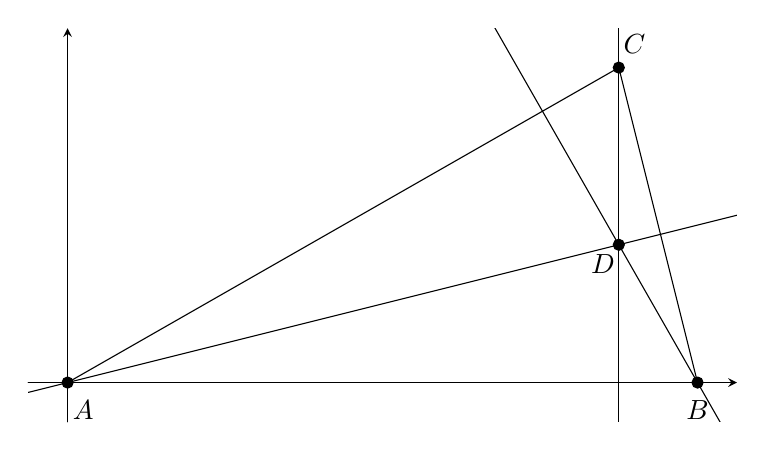
\begin{tikzpicture}[line cap=round,line join=round,>=triangle 45,x=1.0cm,y=1.0cm]
\begin{axis}[
x=1.0cm,y=1.0cm,
axis lines=middle,
ticks=none,
xmin=-0.5,
xmax=8.5,
ymin=-0.5,
ymax=4.5,]
\clip(-0.5,-0.5) rectangle (8.5,4.5);
%\fill[color=black,fill=black,fill opacity=0.10000000149011612] (0.,0.) -- (7.,4.) -- (8.,0.) -- cycle;
\draw  (0.,0.)-- (7.,4.);
\draw  (7.,4.)-- (8.,0.);
\draw  (8.,0.)-- (0.,0.);
\draw  (7.,-0.5) -- (7.,4.5);
\draw [domain=-0.5:8.5] plot(\x,{(-0.--0.25*\x)/1.});
\draw [domain=-0.5:8.5] plot(\x,{(--14.-1.75*\x)/1.});
\begin{scriptsize}
\draw [fill=black] (0.,0.) circle [radius=2.0pt];
\draw (0.2,-0.35) node {$A$};
\draw [fill=black] (7.,4.) circle [radius=2.0pt];
\draw (7.2,4.3) node {$C$};
\draw [fill=black] (8.,0.) circle [radius=2.0pt];
\draw (8.0,-0.35) node {$B$};

\draw [fill=black] (7.,1.75) circle [radius=2.0pt];
\draw[color=black] (6.8,1.5) node {$D$};
\end{scriptsize}
\end{axis}
\end{tikzpicture}
\end{document}
	\caption{Ortocentro triangolo}
	\label{fig:ortocentro1}
\end{figure}
\begin{proof}
Consideriamo un triangolo come nella figura~\cref{fig:ortocentro1}. Poniamo che $A(0,0)$, $B(0,s)$ e $C(t,r)$ otteniamo che  le altezze relative ai lati sono:
\begin{align*}
y=&-\dfrac{t}{r}(x-s)\\
x=&t\\
y=&\dfrac{s-t}{r}x\\
\intertext{mettendo a sistema le prime due otteniamo}
&\begin{cases}
y=-\dfrac{t}{r}(x-s)\\
x=t
\end{cases}\\
\intertext{otteniamo:}
&\begin{cases}
y=\dfrac{t}{r}(s-t)\\
x=t
\end{cases}\\
\intertext{mettendo a sistema le rimanenti otteniamo}
&\begin{cases}
y=\dfrac{s-t}{r}x\\
x=t
\end{cases}\\
\intertext{otteniamo:}
&\begin{cases}
y=\dfrac{t}{r}(s-t)\\
x=t
\end{cases}\\
\end{align*}
\end{proof}
\begin{cor}[Triangolo rettangolo]
Nel triangolo rettangolo l'ortocentro coincide con il vertice dell'angolo retto.
\end{cor}
\begin{proof}
Dal~\cref{thm:ortocentro1} abbiamo 
\begin{align*}
&\begin{cases}
y=\dfrac{t}{r}(s-t)\\
x=t
\end{cases}
\intertext{basta porre $s=t$ per ottenere}
&\begin{cases}
y=0\\
x=s
\end{cases}
\end{align*}
\end{proof}
\section{Baricentro}\label{sec:baricentro}
\begin{defn}[Mediana]\label{defn:mediana1}
	In un triangolo è il segmento che unisce un vertice con il punto medio del lato opposto.\index{Triangolo!mediana}\index{Mediana!triangolo}
\end{defn}
\begin{thm}[Lunghezza mediana]\label{thm:mediana1}
Consideriamo il triangolo in~\cref{fig:mediana1} le mediane hanno lunghezza
\begin{align*}
m_a=&\dfrac{\sqrt{2(b^2+c^2)-a^2}}{2}\\
m_b=&\dfrac{\sqrt{2(a^2+c^2)-b^2}}{2}\\
m_c=&\dfrac{\sqrt{2(a^2+b^2)-c^2}}{2}\\
\end{align*}
\end{thm}
\begin{proof}
Diretta conseguenza del~\cref{cor:ceviana1}
\end{proof}
\begin{figure}
	\centering
	\documentclass[10pt]{standalone}
\usepackage[utf8]{inputenc}
\usepackage{pgf,tikz,pgfplots}
\pgfplotsset{compat=1.15}
\usepackage{mathrsfs}
\usetikzlibrary{arrows}
\pagestyle{empty}
\begin{document}

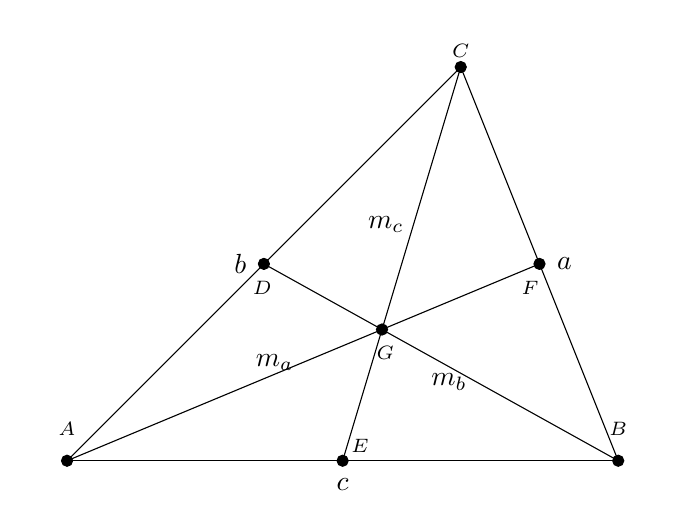
\begin{tikzpicture}[line cap=round,line join=round,>=triangle 45,x=1.0cm,y=1.0cm]

\clip(-0.5,-0.5) rectangle (7.5,5.5);
%\fill[line width=2.pt,color=black,fill=black,fill opacity=0.10000000149011612] (0.,0.) -- (7.,0.) -- (5.,5.) -- cycle;
\draw  (0.,0.)-- (7.,0.)node [midway,below=0.1cm] {$c$};
\draw  (7.,0.)-- (5.,5.)node [midway,right=0.1cm] {$a$};
\draw  (5.,5.)-- (0.,0.)node [midway,left=0.1cm] {$b$};
\draw  (0.,0.)-- (6.,2.5)node [pos=0.5,left] {$m_a$};
\draw  (7.,0.)-- (2.5,2.5)node [pos=0.4,left] {$m_b$};
\draw  (3.5,0.)-- (5.,5.)node [pos=0.6,left] {$m_c$};
\begin{scriptsize}
\draw [fill=black] (0.,0.) circle (2.0pt);
\draw (0.0,0.4) node {$A$};
\draw [fill=black] (7.,0.) circle (2.0pt);
\draw (7.0,0.4) node {$B$};
\draw [fill=black] (5.,5.) circle (2.0pt);
\draw (5.0,5.2) node {$C$};
\draw [fill=black] (2.5,2.5) circle (2.0pt);
\draw (2.48,2.19) node {$D$};
\draw [fill=black] (3.5,0.) circle (2.0pt);
\draw (3.72,0.19) node {$E$};
\draw [fill=black] (6.,2.5) circle (2.0pt);
\draw (5.88,2.19) node {$F$};

\draw [fill=black] (4.,1.6666666666666667) circle (2.0pt);
\draw (4.04,1.37) node {$G$};
\end{scriptsize}
\end{tikzpicture}
\end{document}
	\caption{Lunghezza mediane}
	\label{fig:mediana1}
\end{figure}
 \begin{defn}[Baricentro]\label{defn:baricentro1}
	Il Baricentro è il punto di intersezione delle mediane di un triangolo \index{Triangolo!baricentro}\index{Baricentro!triangolo}
\end{defn}
\begin{thm}[Coordinate baricentro]\label{thm:baricentro1}
	In un triangolo di vertici $A(a,b)$, $B(c,d)$ e $C(e,f)$ il baricentro $M$ ha coordinate\[M\left(\frac{a+c+e}{3},\frac{b+d+f}{3}\right)\]
\end{thm}\index{Triangolo!baricentro!coordinate}\index{Baricentro!coordinate}	
\begin{proof}
Consideriamo il triangolo della~\cref{fig:baricentro1} e determiniamo le mediane
\begin{align*}
\intertext{La mediana $AF$ ha equazione}
y =& x\dfrac{2b-d-f}{2a-c-e}+\dfrac{a(d+f)-b(c+e)}{2a-c-e}\\
\intertext{La mediana $BD$ ha equazione}
y =& x\dfrac{b - 2d + f}{a - 2c + e} +\dfrac{d(a+e)-c(b+f)}{a - 2c + e}\\
\intertext{Per trovare il punto $M$ di intersezione le metto a sistema}
&\begin{cases}
y = x\dfrac{2b-d-f}{2a-c- e}+\dfrac{a(d+f)-b(c+e)}{2a-c-e}\\ \\
y = x\dfrac{b - 2d + f}{a - 2c + e}+\dfrac{d(a+e)-c(b+f)}{a-2c+e}
\end{cases}
\intertext{che risolto mi da}
&\begin{cases}
x=\dfrac{a+c+e}{3}\\ \\
y=\dfrac{b+d+f}{3}
\end{cases}
\end{align*}
Da cui la tesi
\end{proof}
\begin{figure}
	\centering
	\documentclass[10pt]{standalone}
\usepackage[utf8]{inputenc}
\usepackage{pgf,tikz,pgfplots}
\pgfplotsset{compat=1.15}
\usepackage{mathrsfs}
\usetikzlibrary{arrows}
\pagestyle{empty}
\begin{document}

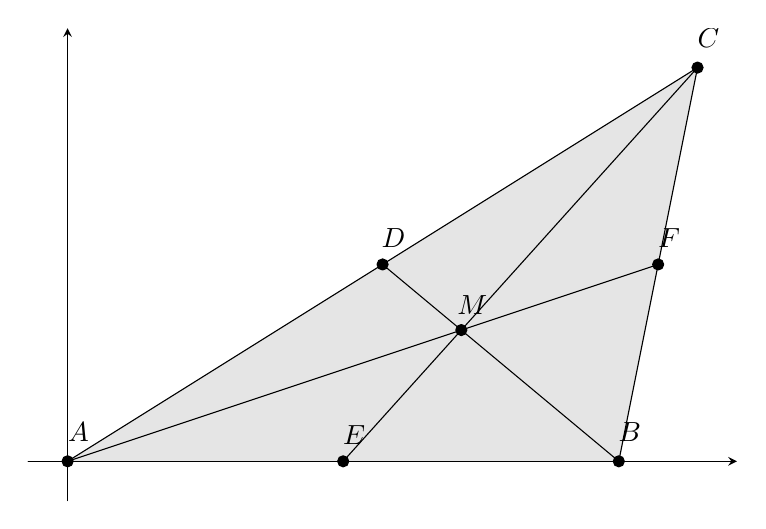
\begin{tikzpicture}[line cap=round,line join=round,>=triangle 45,x=1.0cm,y=1.0cm]
\begin{axis}[
x=1.0cm,y=1.0cm,
axis lines=middle,
xmin=-0.5,
xmax=8.5,
ymin=-0.5,
ymax=5.5,
ticks=none,
]
\clip(-0.5,-0.5) rectangle (8.5,5.5);
\fill[,color=black,fill=black,fill opacity=0.1] (0.,0.) -- (7.,0.) -- (8.,5.) -- cycle;
\draw  (0.,0.)-- (7.,0.);
\draw  (7.,0.)-- (8.,5.);
\draw  (8.,5.)-- (0.,0.);
\draw  (0.,0.)-- (7.5,2.5);
\draw (7.,0.)-- (4.,2.5);
\draw (3.5,0.)-- (8.,5.);
\begin{scriptsize}
\draw [fill=black] (0.,0.) circle (2.0pt);
\draw[color=black] (0.14,0.37) node {$A$};
\draw [fill=black] (7.,0.) circle (2.0pt);
\draw[color=black] (7.14,0.37) node {$B$};
\draw [fill=black] (8.,5.) circle (2.0pt);
\draw[color=black] (8.14,5.37) node {$C$};

\draw [fill=black] (4.,2.5) circle (2.0pt);
\draw[color=black] (4.14,2.83) node {$D$};
\draw [fill=black] (3.5,0.) circle (2.0pt);
\draw[color=black] (3.64,0.33) node {$E$};
\draw [fill=black] (7.5,2.5) circle (2.0pt);
\draw[color=black] (7.64,2.83) node {$F$};

\draw [fill=black] (5.,1.6666666666666667) circle (2.0pt);
\draw[color=black] (5.14,1.99) node {$M$};
\end{scriptsize}
\end{axis}
\end{tikzpicture}
\end{document}
	\caption{Baricentro di un triangolo}
	\label{fig:baricentro1}
\end{figure}
\begin{thm}[Teorema di Eulero]\label{thm:eulero1}
In un triangolo Ortocentro, Circocentro e Baricentro sono allineati
\end{thm}\index{Triangolo!Eulero}\index{Triangolo!ortocentro}\index{Triangolo!circocentro}\index{Circocentro!triangolo}\index{Ortocentro!triangolo}\index{Baricentro!triangolo}\index{Triangolo!baricentro}
\begin{proof}
	Consideriamo la retta che passa per il circocentro e per l'ortocentro. Utilizzando il~\cref{thm:CircoAsse1} e il~\cref{thm:baricentro1} otteniamo
	\[y=x\dfrac{[r^2-3t(s-t)]}{r(s-2t)}+\dfrac{t[r^2-(s+t)(s-t)]}{r(s-2t)}\]
Adattando il~\cref{thm:baricentro1} il Baricentro ha coordinate: \[M\left(\frac{s+t}{3},\frac{t}{3}\right)\] che verificano l'equazione.
\end{proof}
\begin{defn}[Retta di Eulero]\label{defn:rettaEulero1}
La retta che passa per Ortocentro, Circocentro e Baricentro  chiamata retta di Eulero\end{defn}\index{Retta!Eulero}
\section{Triangolo equilatero}\label{sec:triangolo-equilatero}
\begin{thm}[Ortocentro, circocentro e baricentro]\label{thm:triangoloequilatero1}
In un triangolo equilatero Ortocentro, Circocentro e Baricentro coincidono.
\end{thm}\index{Triangolo!equilatero}\index{Triangolo!equilatero!ortocentro}\index{Triangolo!equilatero!circocentro}\index{Circocentro!triangolo!equilatero}\index{Ortocentro!triangolo!equilatero}\index{Triangolo!baricentro}\index{Triangolo!equilatero!baricentro}
\begin{figure}
	\centering
	\documentclass[10pt]{standalone}
\usepackage[utf8]{inputenc}
\usepackage{pgf,tikz,pgfplots}
\pgfplotsset{compat=1.15}
\usepackage{mathrsfs}
\usetikzlibrary{arrows}
\pagestyle{empty}
\begin{document}

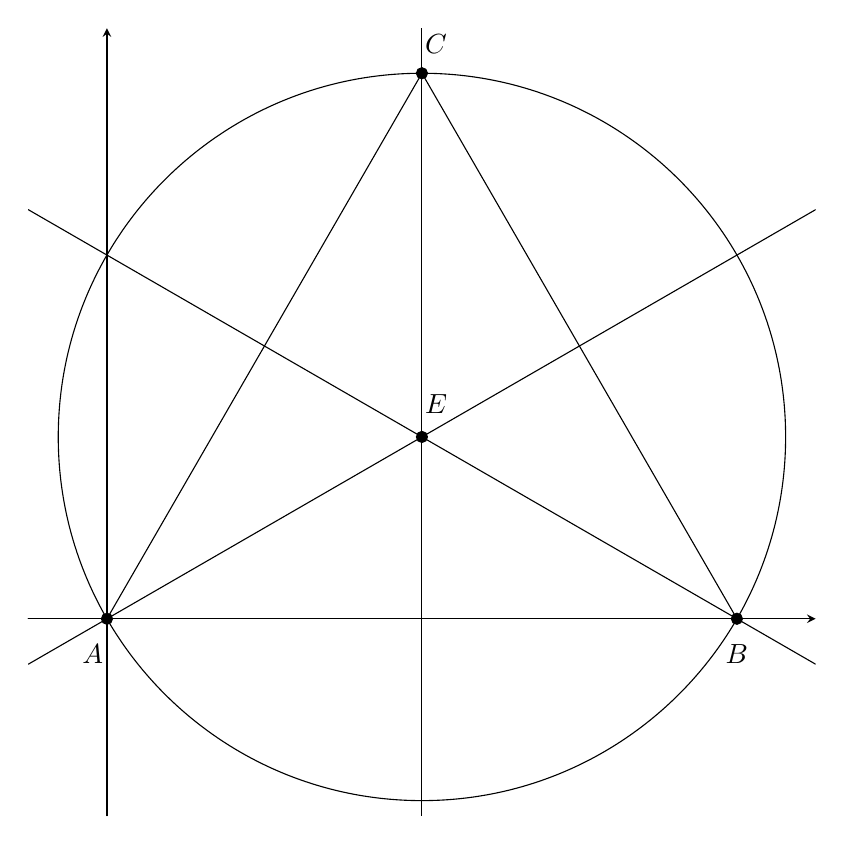
\begin{tikzpicture}[line cap=round,line join=round,>=triangle 45,x=1.0cm,y=1.0cm]
\begin{axis}[
x=1.0cm,y=1.0cm,
axis lines=middle,
%ymajorgrids=true,
%xmajorgrids=true,
xmin=-1.0,
xmax=9.0,
ymin=-2.5,
ymax=7.5,
ticks=none]
\clip(-1.,-2.5) rectangle (9.,7.5);
%\fill[color=black,fill=black,fill opacity=0.1] (0.,0.) -- (8.,0.) -- (4.,6.928203230275509) -- cycle;
\draw  (0.,0.)-- (8.,0.);
\draw  (8.,0.)-- (4.,6.928203230275509);
\draw  (4.,6.928203230275509)-- (0.,0.);
\draw  (4.,2.3094010767585025) circle (4.618802153517006cm);
\draw [domain=-1.:9.] plot(\x,{(--32.-4.*\x)/6.928203230275509});
\draw [domain=-1.:9.] plot(\x,{(-0.-4.*\x)/-6.928203230275509});
\draw  (4.,-2.5) -- (4.,7.5);
\begin{scriptsize}
\draw [fill=black] (0.,0.) circle (2.0pt);
\draw (-0.18,-0.45) node {$A$};
\draw [fill=black] (8.,0.) circle (2.0pt);
\draw (8.0,-0.45) node {$B$};
\draw [fill=black] (4.,6.928203230275509) circle (2.0pt);
\draw (4.18,7.3) node {$C$};

\draw [fill=black] (4.,2.3094010767585025) circle (2.0pt);
\draw (4.18,2.73) node {$E$};
\end{scriptsize}
\end{axis}
\end{tikzpicture}
\end{document}
	\caption{Triangolo equilatero}
	\label{fig:triangoloequilatero1}
\end{figure}
\begin{proof}
	Costruiamo la~\cref{fig:triangoloequilatero1}, un triangolo equilatero di lato $s$. Le coordinate del suoi vertici sono $A(0,0)$, $B(s,0)$ e $C(\frac{s}{2},\frac{s}{2}\sqrt{3})$. 
	Per~\cref{thm:CircoAsse1} le coordinate del circocentro\index{Triangolo!circocentro}\index{Circocentro!triangolo!equilatero} sono
	\[\begin{cases}
	x=\dfrac{s}{2}\\ \\
	y=\dfrac{t^2+r^2-ts}{2r}\\
	\end{cases}\]
	Per il~\cref{thm:ortocentro1} le coordinate dell'ortocentro\index{Triangolo!ortocentro}\index{Ortocentro!triangolo!equilatero} sono \[\begin{cases}
	y=\dfrac{t}{r}(s-t)\\
	x=t
	\end{cases}\] 
	Per il~\cref{thm:baricentro1} le coordinate del baricentro\index{Triangolo!baricentro}\index{Baricentro!triangolo!equilatero} sono \[\begin{cases}
	x=\dfrac{a+c+e}{3}\\ \\
	y=\dfrac{b+d+f}{3}
	\end{cases} \]
	Adattando le tre formule al triangolo equilatero otteniamo:
	\[\begin{cases}
	x=\dfrac{s}{2}\\ \\
	y=\dfrac{s}{6}\sqrt{3}
	\end{cases}\]
\end{proof}
\section{Excentro}\label{sec:excentro}
\begin{defn}[Exentro]\label{defn:excentro}
Si dice excentro  di un triangolo il punto di incontro delle bisettrici di due angoli esterni e della bisettrice dell'angolo interno non adiacente ad essi.
\end{defn}\index{Triangolo!excentro}
\begin{figure}
	\centering
	\documentclass[10pt]{standalone}
\usepackage[utf8]{inputenc}
\usepackage{pgf,tikz,pgfplots}
\pgfplotsset{compat=1.15}
\usepackage{mathrsfs}
\usetikzlibrary{arrows}
\pagestyle{empty}
\begin{document}
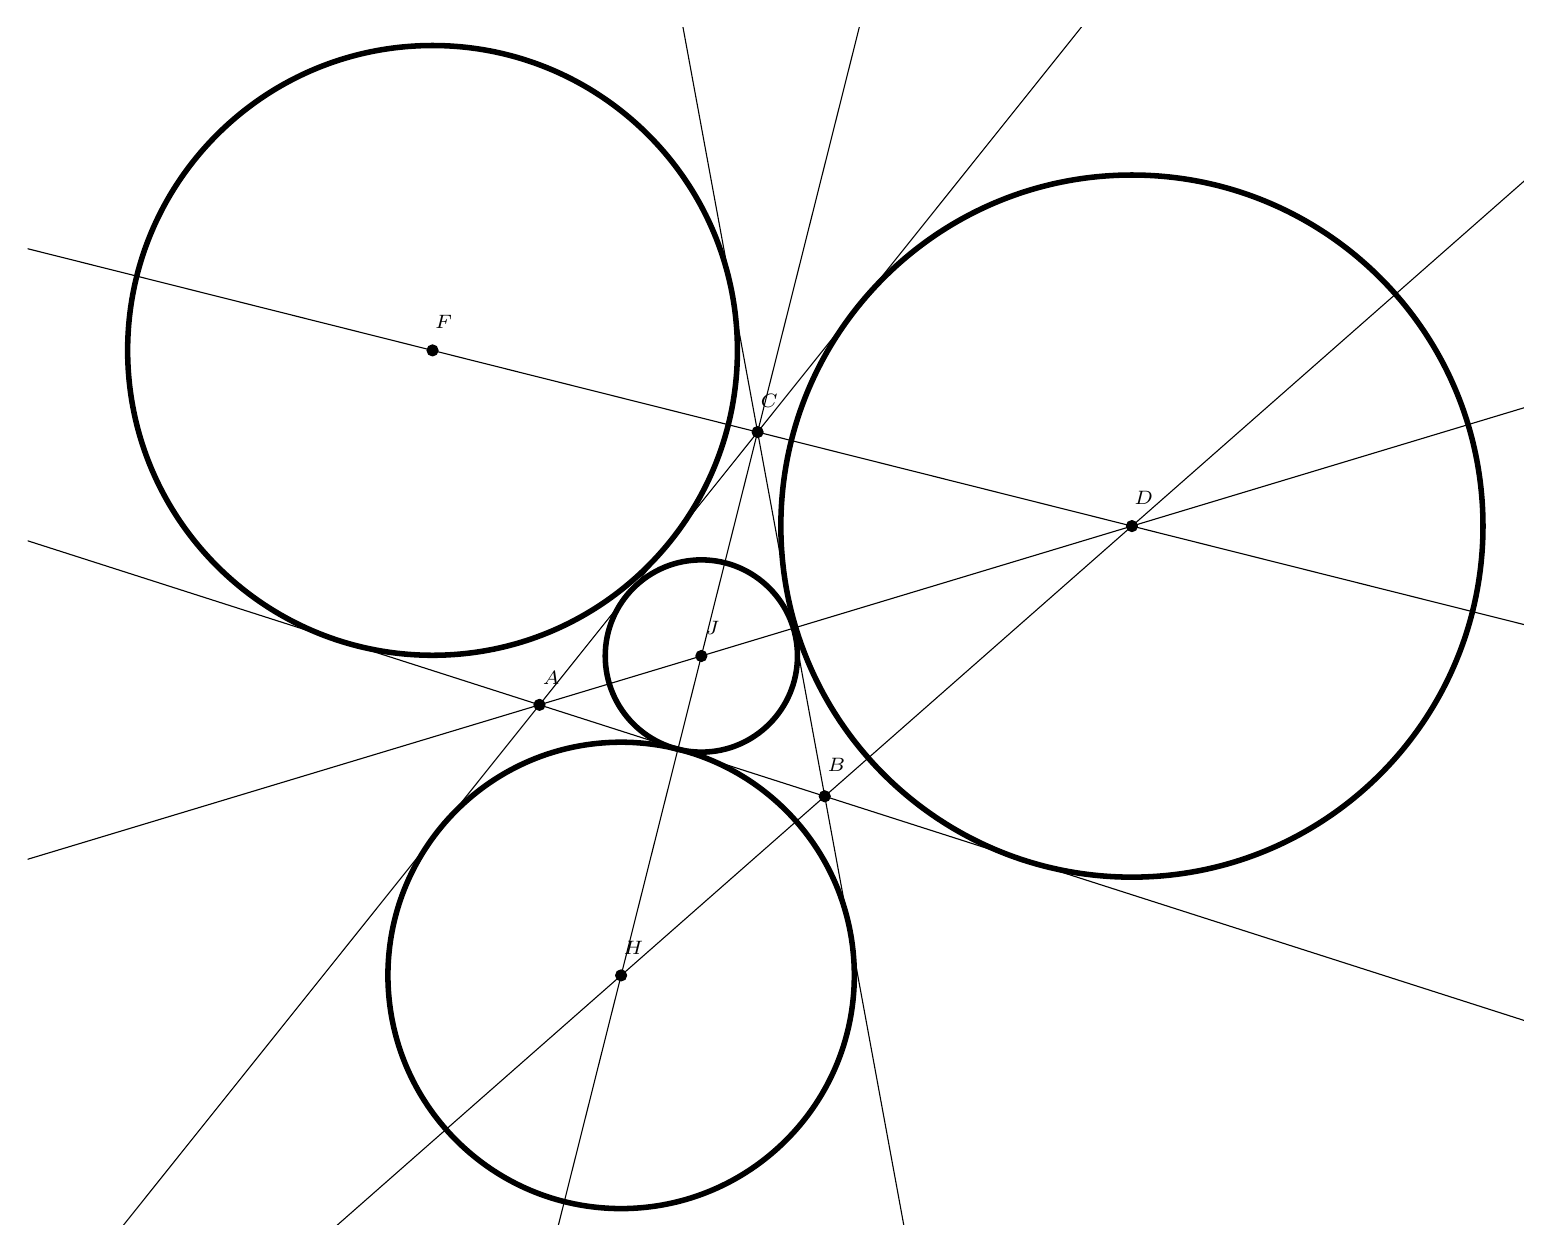
\begin{tikzpicture}[line cap=round,line join=round,>=triangle 45,x=1.0cm,y=1.0cm]
%\begin{axis}[
%x=1.0cm,y=1.0cm,
%axis lines=middle,
%%ymajorgrids=true,
%%xmajorgrids=true,
%xmin=-6.0,
%xmax=12.5,
%ymin=-6.6,
%ymax=8.6,
%ticks=none,
%]
\clip(-6.5,-6.6) rectangle (12.5,8.6);
\draw [domain=-6.5:13.5] plot(\x,{(-0.--3.464396052718255*\x)/2.770130751191044});
\draw [domain=-6.5:13.5] plot(\x,{(--15.767610844916462-4.625656769270266*\x)/0.8526556256719391});
\draw [domain=-6.5:13.5] plot(\x,{(-0.--1.1612607165520117*\x)/-3.622786376862983});
\draw [domain=-6.5:13.5] plot(\x,{(-0.-0.28887520413651546*\x)/-0.9573667617141753});
\draw [domain=-6.5:13.5] plot(\x,{(--3.2646741596274698-0.6604688485205706*\x)/-0.7508534478404635});
\draw [domain=-6.5:13.5] plot(\x,{(--4.034892461887093-0.24362882555343285*\x)/0.9698685454016205});
\draw [domain=-6.5:13.5] plot(\x,{(-1.842635940654259--0.9698685454016205*\x)/0.24362882555343285});
\draw [line width=2.pt] (7.523905849169923,2.270258301208685) circle (4.45854360090309cm);
\draw [line width=2.pt] (-1.3582611636615378,4.501438936940597) circle (3.8719996160129293cm);
\draw [line width=2.pt] (1.036771011839885,-3.435982362041759) circle (2.96160697641247cm);
\draw [line width=2.pt] (2.0556962169911097,0.6202843968206011) circle (1.2206781158240956cm);
\begin{scriptsize}
\draw [fill=black] (0.,0.) circle (2.0pt);
\draw[color=black] (0.1482147022498305,0.34154482369477995) node {$A$};
\draw [fill=black] (3.622786376862983,-1.1612607165520117) circle (2.0pt);
\draw[color=black] (3.7720011113555727,-0.7669074896787401) node {$B$};
\draw [fill=black] (2.770130751191044,3.464396052718255) circle (2.0pt);
\draw[color=black] (2.919345485683633,3.8587492795915264) node {$C$};
\draw [fill=black] (7.523905849169923,2.270258301208685) circle (2.0pt);
\draw[color=black] (7.672900598804695,2.6223986223672155) node {$D$};

\draw [fill=black] (-1.3582611636615378,4.501438936940597) circle (2.0pt);
\draw[color=black] (-1.2160342988252724,4.860619639756054) node {$F$};
;
\draw [fill=black] (1.036771011839885,-3.435982362041759) circle (2.0pt);
\draw[color=black] (1.1927178436979562,-3.0903940696347725) node {$H$};
%\draw [fill=black] (1.7583038412541079,-0.5636129117773052) circle (2.0pt);
%\draw[color=black] (1.9174751255191047,-0.21268133299198008) node {$I$};

\draw [fill=black] (2.0556962169911097,0.6202843968206011) circle (2.0pt);
\draw[color=black] (2.1945882038624847,0.9810365429487338) node {$J$};

\end{scriptsize}
%\end{axis}
\end{tikzpicture}
\end{document}
	\caption{Triangolo e circonferenze tangenti}
	\label{fig:excentro1}
\end{figure}
